\begin{center}
\begin{tikzpicture}
    \node[anchor=south west,inner sep=0] (image)  at (0,0) {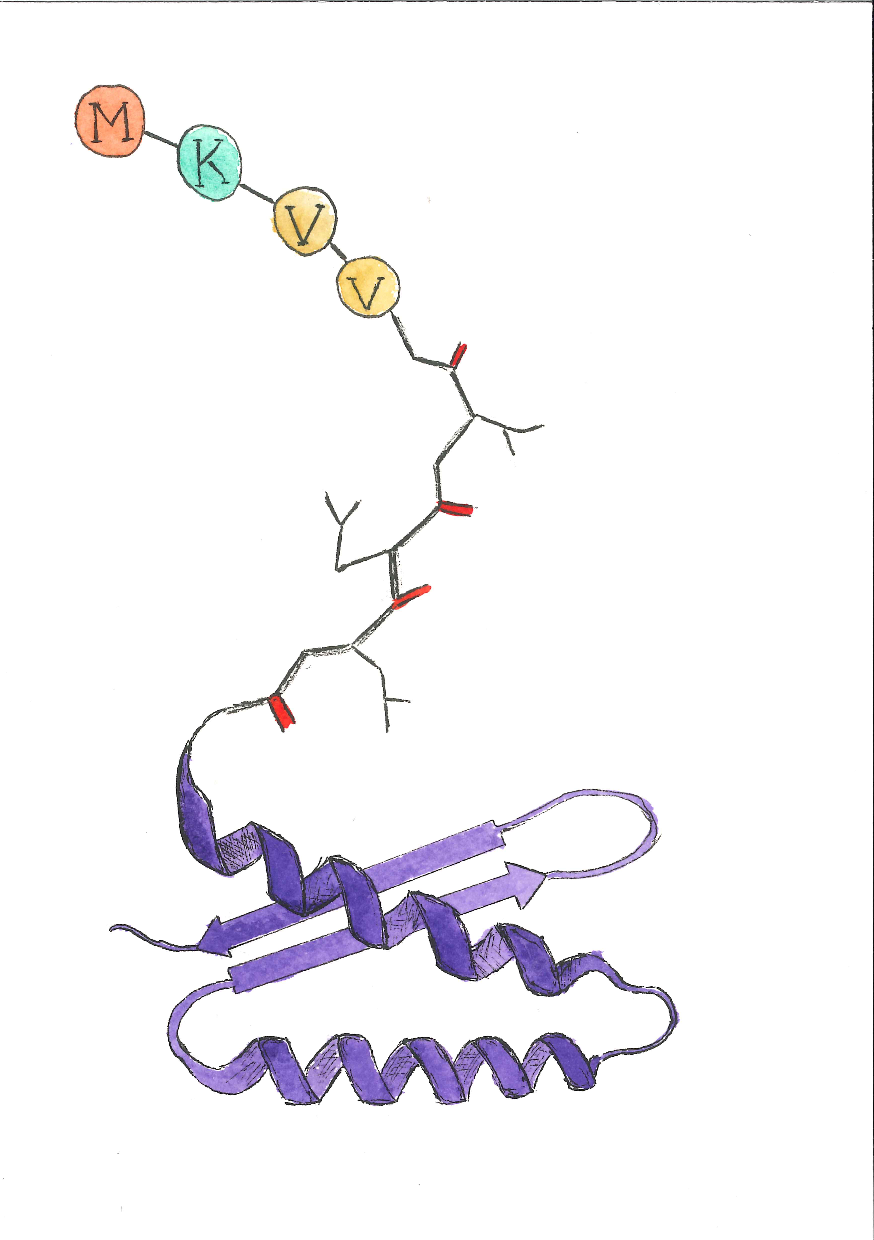
\includegraphics[trim={2mm, 2mm, 2mm, 2mm}, width=0.995\pagewidth]{scans/201909201655.pdf}};
    
   
    \begin{scope}[x={(image.south east)},y={(image.north west)}]
        \if\helplines1
        	\draw[help lines,xstep=.1,ystep=.1] (0,0) grid (1,1);
        \fi
        \node[align=justify, anchor=north west, text width=0.6\pagewidth] at (0.3, 0.95) {\english{Proteins are long chains of individual blocks called amino acids.}};
        \node[align=justify, anchor=north west, text width=0.3\pagewidth] at (0.65, 0.67) {\english{They are all almost identical, except for the branches: the \emph{side-chains}.}};
         \node[align=justify, anchor=north west, text width=0.35\pagewidth] at (0.55, 0.50) {\english{These long chains fold unto themselves, forming complicated structures. The protein is born and it is thus, ready to perform its specific function.}};
         \node[align=center, anchor=north, text width=0.4\pagewidth] at (0.3, 0.09) {\english{We want to know how to get from the sequence of amino acids to the 3D structure.}};
         
         % % % %
        \node[align=left, anchor=north west, text width=0.5\pagewidth] at (0.45, 0.85) {\spanish{Las proteínas son largas cadenas cuyos eslabones se llaman aminoácidos.}};
        
        \node[align=justify, anchor=north west, text width=0.3\pagewidth] at (0.1, 0.7) {\spanish{Son todos casi idénticos, excepto por las ramas: las \emph{cadenas laterales}.}};
        
        \node[align=justify, anchor=north west, text width=0.3\pagewidth] at (0.04, 0.60) {\spanish{Cuando estas cadenas se pliegan sobre sí mismas en estructuras complicadas, tenemos una proteína capaz de realizar una función concreta.}};
        
        \node[align=center, anchor=north , text width=0.4\pagewidth] at (0.7, 0.09) {\spanish{Queremos saber cómo ir de la secuencia de aminoácidos a esta estructura en \oldstylenums{3}\textsc{d}.}};
        
    \end{scope}

\end{tikzpicture}
\end{center}